\documentclass[11pt]{article}
\usepackage[margin=1in]{geometry}
\usepackage{amsmath,amssymb,amsthm,booktabs,graphicx}
\usepackage[colorlinks=true,linkcolor=blue,citecolor=blue,urlcolor=blue]{hyperref}
\setlength{\emergencystretch}{2em}
\newtheorem{theorem}{Theorem}[section]
\newtheorem{lemma}[theorem]{Lemma}
\newtheorem{corollary}[theorem]{Corollary}
\newtheorem{proposition}[theorem]{Proposition}
\theoremstyle{remark}\newtheorem{remark}[theorem]{Remark}
\newcommand{\R}{\mathbb R}\newcommand{\C}{\mathbb C}
\newcommand{\Rea}{\operatorname{Re}}\newcommand{\Ima}{\operatorname{Im}}
\newcommand{\diag}{\operatorname{diag}}
\title{Granularity and stability at coordinate interfaces\\
\large Static thresholds, planar response sets, and finite-rate instability}
\author{}
\date{27 September 2026}
\begin{document}
\maketitle
\begin{abstract}
Positive first-order attachments to a single coordinate of a D-stable matrix
have an exact distribution-free stability threshold: the first static
D-instability along the corresponding positive diagonal ray. Below this
threshold every finite positive partition is D-stable; at the threshold
only a zero eigenvalue can obstruct stability; above it every sufficiently
fine partition admits strict growth. This is an exact reduction to a static
D-stability problem, not an arbitrary-dimensional decision procedure.
We give a direct closed-right-half-plane absorption identity and a finite
construction preserving an unstable eigenvalue. These yield quantitative
partition bounds without a contour-limit argument. Planar response geometry
also gives an exact test for a fixed partition. We extend safety to several
coordinate ports and reciprocal relaxation modules, explain the relation to
negative-imaginary systems, and show that four core states are necessary and
sufficient for fixed-total granularity sensitivity. Exact rational examples
distinguish stable and unstable two-piece partitions at the same total load.
The single-port threshold theorem is verified end-to-end in Lean;
the scope of the additional conventional proofs is stated in
Section~\ref{sec:formal}.
\end{abstract}

\section{Problem and scope}
A real square matrix is \emph{Hurwitz} if all its eigenvalues have strictly
negative real part, and \emph{D-stable} if $DB$ is Hurwitz for every positive
diagonal $D$. Left and right scaling have the same spectra, since
$DB=D(BD)D^{-1}$. We distinguish strict instability, meaning an eigenvalue in
$\Rea z>0$, from a marginal eigenvalue on the imaginary axis.

Fix a D-stable $n\times n$ matrix $B$, a coordinate vector $e=e_p$, and a
finite nonempty partition $r=(r_1,\ldots,r_m)$ with $r_j>0$. Write
\begin{equation}\label{eq:attached}
 A_r=\begin{pmatrix}B&er^T\\\mathbf1e^T&-I_m\end{pmatrix},
 \qquad G=\sum_jr_j,\qquad B_X=B+Xee^T.
\end{equation}
Every core and attachment rate is free and positive. A scalar attachment
with damping $h_j>0$ and positive forward and return gains $a_j,c_j$ has
normalized load $r_j=a_jc_j/h_j$: a positive diagonal coordinate change and
a reparameterization of its row rate give \eqref{eq:attached}.

The question is how D-stability depends on the distribution of a fixed $G$.
The answer retains the entire static loading interval. D-stability is not
monotone under diagonal changes, and stable endpoints do not imply stability
between them. Our results concern this restricted interface architecture;
they do not settle the general characterization of D-stable matrices.

Schur complements, Routh--Hurwitz criteria, continuity of polynomial roots,
and zero exclusion are classical ingredients \cite{barmish,cross}.
The dynamic-to-static reduction below uses the freedom of the rate at the
\emph{same coordinate} to which the attachments couple. That assumption is
essential to the proof.

\section{Direct spectral absorption}
Inverse rates are convenient: $z$ is an eigenvalue of $DA$ precisely when
$(zQ-A)v=0$ for $Q=D^{-1}>0$ and a nonzero vector $v$.

\begin{lemma}[Closed-half-plane absorption]\label{lem:absorb}
Let $z=\sigma+i\omega\ne0$, $\sigma\ge0$, and $r,t>0$. Set
\begin{equation}\label{eq:absorb}
 d=(1+\sigma t)^2+\omega^2t^2,\qquad
 \alpha=\frac{rt}{d},\qquad x=\frac{r(1+2\sigma t)}{d}.
\end{equation}
Then $\alpha>0$, $0<x<r$, and
\begin{equation}\label{eq:identity}
 \frac{r}{1+zt}+z\alpha=x.
\end{equation}
\end{lemma}
\begin{proof}
The denominator is positive. Multiplication by the complex conjugate proves
\eqref{eq:identity}; moreover
$r-x=r|z|^2t^2/d>0$ and $1+2\sigma t>0$.
\end{proof}

\begin{theorem}[Static-interval safety]\label{thm:safety}
Suppose $B_X$ is D-stable for every $0<X<G$. Then every positive partition
of $G$ has no nonzero eigenvalue in the closed right half-plane under any
positive scaling. It is D-stable if and only if $\det B_G\ne0$.
If $\det B_G=0$, its only possible eigenvalues outside the strict left
half-plane are zero eigenvalues.
\end{theorem}
\begin{proof}
For a nonzero candidate $z$ with $\Rea z\ge0$, every $1+zt_j$ is nonzero.
Eliminating the leaves gives
\[
 \left(zQ-B-ee^T\sum_j\frac{r_j}{1+zt_j}\right)v=0.
\]
The core vector $v$ is nonzero, since a zero core vector would force every
leaf coordinate to vanish. Apply Lemma~\ref{lem:absorb} termwise. With
$X=\sum_jx_j\in(0,G)$ and
$Q'=Q+(\sum_j\alpha_j)ee^T>0$, the same equation is
$(zQ'-B_X)v=0$, contradicting D-stability of $B_X$.
At $z=0$, ordinary block elimination gives
$\det(-A_r)=\det(-B_G)$. Positive scaling multiplies the determinant
by a positive factor, so occurrence of a zero eigenvalue is independent
of the partition and rates.
\end{proof}

This proof includes real positive eigenvalues and does not require spectral
continuation or stability of the principal block obtained by deleting $p$.
At $\sigma=0$ it is the familiar phase absorption
$X=\sum r_j/(1+t_j^2)$ and $q'_p=q_p+\sum r_jt_j/(1+t_j^2)$.

\section{The exact threshold and finite realization}
Define
\begin{equation}\label{eq:tau}
 \tau=\inf\{X\ge0:\ B_X\text{ has a strictly unstable positive scaling}\}.
\end{equation}
The infimum is finite: D-stability implies $B_{pp}\le0$, while
$X>-B_{pp}$ makes the port diagonal positive. Increasing its positive
column scaling makes the trace positive, forcing an eigenvalue with
positive real part. Thus $0\le\tau\le-B_{pp}$.

\begin{lemma}[Static marginality below first strict growth]\label{lem:marginal}
$B_X$ is D-stable for $0\le X<\tau$.
\end{lemma}
\begin{proof}
Strict growth is excluded by definition, and $X=0$ is covered by the
hypothesis on $B$. Suppose a positive load $X$ has a contact $i\omega$
at inverse rates $Q>0$. Put $P(z)=zQ-B$ and
$c(z)=\operatorname{adj}(P(z))_{pp}$. Affineness of the determinant gives
$\det(P(i\omega)-Xee^T)=\det P(i\omega)-Xc(i\omega)=0$.
The unloaded determinant is nonzero by D-stability, hence $c(i\omega)\ne0$.
The continuous quotient $f(z)=\det P(z)/c(z)$ is therefore defined near
the contact and satisfies $f(i\omega)=X$.

For small $\sigma>0$, set $z=\sigma+i\omega$ and, if $\omega\ne0$, put
\[
 k(\sigma)=-\frac{\Ima f(z)}{\omega},\qquad
 Y(\sigma)=\Rea f(z)+\sigma k(\sigma).
\]
If $\omega=0$, use $k(\sigma)=0$ and $Y(\sigma)=f(\sigma)$, which is real.
In either case $k(\sigma)\to0$, $Y(\sigma)\to X$, and
$f(z)+zk(\sigma)-Y(\sigma)=0$. Changing just the port inverse rate to
$q_p+k(\sigma)$ and the load to $Y(\sigma)$ thus makes the determinant
zero at $z$, while preserving positive rates and positive load for small
$\sigma$. This produces strict growth arbitrarily close to $X$, and
therefore $\tau\le X$, a contradiction.
\end{proof}

\begin{lemma}[Finite realization of static growth]\label{lem:finite}
Suppose $0<X<G$ and $B_X$ has an eigenvalue $z=\sigma+i\omega$, $\sigma>0$,
at positive inverse core rates $Q$. There is $\varepsilon>0$ such that
every partition of $G$ with $\max_jr_j<\varepsilon$ realizes exactly this
eigenvalue at finite positive rates.
\end{lemma}
\begin{proof}
Let $q=Q_{pp}$, $k=|z|^2$, and
\[
 f(t)=\frac{1+2\sigma t}{1+2\sigma t+kt^2}.
\]
This function decreases continuously from $1$ to $0$ on $(0,\infty)$:
$f'(t)=-2kt(1+\sigma t)/(1+2\sigma t+kt^2)^2<0$.
Choose $\delta>0$ satisfying
\begin{equation}\label{eq:quant}
 G\delta+\frac{Gk\delta^2}{2\sigma}<q,\qquad
 Gk\delta^2<G-X,
\end{equation}
and choose
$0<\varepsilon<\min\{G-X,X[1-f(\delta)]\}$.
The first partial sum $S$ strictly greater than $X$ obeys
$X<S<X+\varepsilon<G$. Give these leaves inverse rate $\delta$.
The remaining leaves receive a common inverse rate $T$ determined by
\begin{equation}\label{eq:T}
 f(T)=y:=\frac{X-Sf(\delta)}{G-S}.
\end{equation}
Here $y>0$ follows from $S-X<X[1-f(\delta)]$.
Also $S[1-f(\delta)]\le Gk\delta^2<G-X$, which proves $y<1$.
Thus a unique finite $T>0$ exists; explicitly
\[
 T=\frac{\sigma(1-y)+\sqrt{\sigma^2(1-y)^2+ky(1-y)}}{ky}.
\]
The total effective static load in \eqref{eq:absorb} is exactly $X$.
The fast leaves contribute at most $G\delta$ to $\sum\alpha_j$.
For each slow leaf, $\alpha_j\le x_j/(2\sigma)$, so their contribution
is at most $X[1-f(\delta)]/(2\sigma)\le Gk\delta^2/(2\sigma)$.
By \eqref{eq:quant} the total is strictly below $q$.
Replace the core hub inverse rate by $q-\sum\alpha_j>0$, retain every
other core inverse rate, and reverse \eqref{eq:identity}. Reconstructing
the leaf eigenvector gives a nonzero eigenvector of the attached matrix
at precisely $z$. All rates are finite.
\end{proof}

\begin{theorem}[Exact distribution-free granularity threshold]\label{thm:threshold}
For \eqref{eq:attached} and \eqref{eq:tau}:
\begin{enumerate}
\item If $0<G<\tau$, every positive partition is D-stable.
\item If $G=\tau>0$, every partition is D-stable exactly when
$\det B_\tau\ne0$. Otherwise only zero eigenvalues can accompany its
strictly left-half-plane spectrum.
\item If $G>\tau$, every sufficiently fine partition has a strictly
unstable positive scaling.
\end{enumerate}
\end{theorem}
\begin{proof}
Lemma~\ref{lem:marginal} and Theorem~\ref{thm:safety} prove the first two
claims; below $\tau$ the determinant is nonzero by the same lemma.
For $G>\tau$, the defining infimum supplies a strictly unstable static
load $X\in(0,G)$. Apply Lemma~\ref{lem:finite}.
\end{proof}

The quantity $\tau$ is explicit only when the static problem can be solved.
The theorem is a reduction, not a claim that evaluating the infimum is easy.
Equations~\eqref{eq:quant}--\eqref{eq:T} give a constructive fineness bound
from any known static witness, without optimizing its rate spread.

\section{Planar geometry and fixed partitions}
\subsection{A hub connecting stable modules}
Consider a hub of self-coefficient $b$ and modules $M_j$ with input $w_j$
and return $c_j^T$. Assume every $M_j$ is D-stable. Define
\[
 V_j=\{c_j^T(iQ_j-M_j)^{-1}w_j:Q_j>0\text{ diagonal}\},
 \qquad G_j=c_j^T(-M_j)^{-1}w_j.
\]
Frequency normalization is legitimate because all positive diagonal rates
are free. It does not assert that $V_j$ is closed under complex scalar
multiplication.

\begin{theorem}[Hub value-set criterion]\label{thm:hub}
The full hub-and-module matrix is D-stable if and only if
\[
 -b-\sum_jG_j>0,\qquad
 \left(\sum_jV_j\right)\cap\{-b+iq:q>0\}=\varnothing.
\]
\end{theorem}
\begin{proof}
Every module pencil on the imaginary axis is invertible. Schur elimination
at frequency one gives $iq_h-b-\sum_jH_j=0$. Since $q_h>0$ is free,
this is exactly intersection with the stated ray. At zero,
$\det(-A)=\prod_j\det(-M_j)(-b-\sum_jG_j)$.
Necessity follows from Hurwitz stability and positivity of these determinants.

For sufficiency, fix positive module rates and let the hub rate tend to
zero. At zero hub rate the modules have strictly stable eigenvalues and
there is one simple zero eigenvalue. The derivative of that eigenvalue
with respect to hub rate is $b+\sum_jG_j<0$, as follows by differentiating
the scalar Schur equation and the simple-root implicit-function theorem.
Thus a Hurwitz scaling exists. The positive
diagonal cone is path connected. Along any compact path, eigenvalues are
bounded and continuous as a multiset; leaving the Hurwitz region requires
a zero or nonzero imaginary root. Both have been excluded.
\end{proof}

In particular, if every $V_j$ lies in the closed lower half-plane, the
positive DC margin alone is necessary and sufficient. An oscillatory
loss through this architecture requires at least one module capable of
positive imaginary response. The positive DC margin supplies the base
point even for nonreciprocal D-stable modules; reciprocity is unnecessary
for this particular step.

\subsection{The exact protection envelope}
For scalar positive leaves, write
\[
 \sum_j\frac{r_j}{1+it_j}=X-iY.
\]
For $0<X<G$ define
\begin{equation}\label{eq:envelope}
 \Lambda_r(X)=\min_{\substack{1\le k\le m,\ S\subseteq\{1,\ldots,m\}\setminus\{k\}\\
 r(S)\le X\le r(S)+r_k}}
 \sqrt{(X-r(S))(r(S)+r_k-X)}.
\end{equation}
The notation in the minimum means that $k$ is an index and $S$ is a
subset of the remaining indices; $r(S)=\sum_{j\in S}r_j$.

\begin{lemma}[Exact leaf image]\label{lem:image}
For one leaf, $Y=\sqrt{X(G-X)}$. For at least two leaves the finite-rate
heights at fixed $X$ are exactly
\[
 \Lambda_r(X)<Y\le\sqrt{X(G-X)}.
\]
\end{lemma}
\begin{proof}
One leaf has $x=r/(1+t^2)$ and $y=\sqrt{x(r-x)}$.
On the slice $0\le x_j\le r_j$, $\sum x_j=X$, the sum of these strictly
concave heights has its maximum at $x_j=r_jX/G$, by concavity and
homogeneity. Its minimum is achieved at a polytope vertex, where at most
one coordinate is not an endpoint. These vertices give \eqref{eq:envelope}.
With at least two leaves a point with every coordinate interior cannot
minimize a strictly concave function. The segment from a minimizing vertex
to the synchronized maximum lies in the interior except at its initial
point and realizes all intermediate heights. Finally $t_j=y_j/x_j>0$
reconstructs finite rates.
\end{proof}

For a D-stable core $B=\left(\begin{smallmatrix}b&a^T\\c&C\end{smallmatrix}\right)$,
put $Z(Q_c)=a^T(iQ_c-C)^{-1}c$ wherever the inverse exists, and define the
extended envelope
\[
 Q^*(X)=\sup\{\Ima Z(Q_c):Q_c>0,\ \Rea Z(Q_c)=-b-X\},
 \quad \sup\varnothing=-\infty.
\]

\begin{theorem}[Exact fixed-partition test]\label{thm:partition}
$A_r$ is D-stable if and only if
\begin{equation}\label{eq:partitiontest}
 \frac{\det(-B_G)}{\det(-B)}>0,
 \qquad Q^*(X)\le\Lambda_r(X)\quad(0<X<G).
\end{equation}
For one leaf use $\Lambda_r(X)=\sqrt{X(G-X)}$.
\end{theorem}
\begin{proof}
An imaginary contact requires $q_h=\Ima Z-Y>0$ and
$X=-b-\Rea Z$. Lemma~\ref{lem:image} shows that such a contact exists
exactly when $Q^*(X)>\Lambda_r(X)$ for some $X$.
The strict inequality is essential: $q_h=0$ is not an admissible rate,
and for multiple leaves the lower height is only a limiting value.

Singular inner pencils lose no contacts in this argument. If
$d=\det(iQ_c-C)=0$, put $n=a^T\operatorname{adj}(iQ_c-C)c$.
The core determinant equals $(iq_h-b)d-n=-n$, hence $n\ne0$ because
$B$ is D-stable. Adding leaves changes only the coefficient of $d$ and
cannot make the determinant vanish.

For a stable base point choose fixed positive core rates and give all
leaves rate $\epsilon$. The fast eigenvalues converge to those of the
stable core. Schur elimination with $z=\epsilon\mu$ shows that the slow
eigenvalues, divided by $\epsilon$, converge to
those of $-I+k\mathbf1r^T$, where $k=e^T(-B)^{-1}e$.
They are $-1$ and $-1+kG$. The determinant condition is $1-kG>0$,
so small positive $\epsilon$ gives a Hurwitz base point. Zero exclusion
along the positive rate cone proves sufficiency. Necessity of the
determinant sign and of contact exclusion is immediate.
\end{proof}

The exact test may require exponentially many subset labels and a difficult
core-envelope computation. Planar geometry does not remove those costs.
For negative-load leaves the maximum positive imaginary height at fixed
negative real response is attained with synchronized times and depends
only on total absolute load. The same contact and base-point reasoning
therefore makes their all-rate classification independent of partition.
Positive leaves differ because their \emph{minimum} protective height is
partition dependent.

\section{Several ports and reciprocal attachments}
Let $P$ be a set of distinct coordinates, each with positive total $G_p$,
and put $B_X=B+\sum_{p\in P}X_pe_pe_p^T$ and
$\mathcal U=\prod_{p\in P}(0,G_p)$.

\begin{theorem}[Open-box criterion]\label{thm:box}
Every choice of positive finite partitions at the ports is D-stable if
and only if every $B_X$, $X\in\mathcal U$, has no strictly unstable
positive scaling and $\det B_G\ne0$.
\end{theorem}
\begin{proof}
First, absence of strict growth on the open box implies D-stability there.
For fixed $Q>0$, $\det(iQ-B_X)$ is multiaffine in $X$. At a zero, a
nonzero coordinate partial allows the one-coordinate perturbation in
Lemma~\ref{lem:marginal}, producing nearby strict growth inside the box.
Thus all coordinate partials vanish at every zero. Affineness propagates
the zero along each coordinate line in the box; the argument is reapplied
at every point reached. Iterating through the coordinates makes the
determinant identically zero, contradicting its limiting value at $X=0$.
For zero frequency, $\det(-B_X)\ge0$ under no strict growth: a negative
constant term would produce a positive real root. A nonnegative affine
function vanishing at an interior point has zero slope. The same
propagation contradicts $\det(-B)>0$.

Apply Lemma~\ref{lem:absorb} independently at all ports. Every nonzero
closed-right-half-plane candidate maps into $\mathcal U$, where it is
excluded. The total-load determinant handles zero.

Conversely, strict growth at an interior $X$ is realized by sufficiently
fine partitions: use Lemma~\ref{lem:finite} independently at every port,
preserving the same eigenvalue and subtracting the respective inverse-rate
shifts. If the total-load determinant vanishes, every partition is singular.
Strict growth on a face also persists at nearby interior points by openness,
but no assumption of stability on all faces is required.
\end{proof}

\begin{corollary}[Reciprocal relaxation safety]\label{cor:relax}
A module with dynamics $\dot z=D_z(Mz+wx_p)$ and return $\alpha w^Tz$,
where $M=M^T<0$ and $\alpha>0$, obeys the same safety conclusions with
total load $G=\alpha w^T(-M)^{-1}w$. Multiple such modules can be combined
at one or several coordinate ports.
\end{corollary}
\begin{proof}
Let $S=D_z^{1/2}MD_z^{1/2}<0$ and $u=D_z^{1/2}w$.
The spectral theorem gives
\[
 H(s)=\alpha u^T(sI-S)^{-1}u
     =\sum_\ell\frac{a_\ell}{s+\lambda_\ell}
     =\sum_\ell\frac{g_\ell}{1+s/\lambda_\ell},
 \quad a_\ell\ge0,\quad\lambda_\ell>0,
\]
where $\sum g_\ell=H(0)=G$ independently of $D_z$.
Omit zero residues and apply the scalar absorption argument at each
fixed scaling. The internal poles are strictly negative.
\end{proof}

For a positive diagonal symmetrizer $H_0$ with $H_0M$ symmetric negative
definite, the reciprocal output must be $\alpha w^TH_0$. Conservation
zero modes require separate treatment. The corollary is a safety result;
its converse does not permit independently tuning the modal rates of a
fixed indivisible subnetwork.

These are classical relaxation transfer functions in the sense of Willems
\cite{willems,chaffey}. Lanzon and Petersen's negative-imaginary theorem
\cite{lanzon} likewise decides an appropriate feedback interconnection by
its DC loop gain. Here the arbitrary core transfer is not assumed to be
negative imaginary for every diagonal scaling. Coordinate-rate absorption,
and the \emph{first} static loss rather than a single endpoint DC test,
are what allow the present threshold theorem to retain static reentry.

\section{Small cores and the minimum dimension}
For a two-state D-stable core
$B=\left(\begin{smallmatrix}-a&p\\q&-b\end{smallmatrix}\right)$, let
$t=ab-pq>0$. Then
\[
 \tau=\begin{cases}\min\{a,t/b\},&b>0,\\a,&b=0.\end{cases}
\]
At positive threshold equality is safe precisely when $t-b\tau>0$.

For three states define signed principal-minor data
\[
 a=-B_{11},\ b=-B_{22},\ c=-B_{33},\quad
 u=\det B_{12},\ v=\det B_{13},\ w=\det B_{23},\ t=\det(-B)>0.
\]
These are nonnegative except that $t$ is strictly positive. For loading
coordinate one put
\[
 L=\min\bigl(\{a\}\cup\{u/b:b>0\}\cup\{v/c:c>0\}\cup\{t/w:w>0\}\bigr),
\]
and, on $[0,L]$, set
$A=w(a-X)$, $E_2=b(v-cX)$, $E_3=c(u-bX)$, and $T=t-wX$.
The classical cubic principal-minor criterion for absence of strict growth is
\begin{equation}\label{eq:cubic}
 T\le(\sqrt A+\sqrt{E_2}+\sqrt{E_3})^2.
\end{equation}
For completeness, the rate-dependent cubic Hurwitz inequality is
$(\sum a_i d_i)(\sum u_{ij}d_id_j)\ge t d_1d_2d_3$.
After division by the positive product, its infimum is the squared sum
in \eqref{eq:cubic}, by Cauchy--Schwarz; zero coefficients are obtained
by limits. A strict violation is realized at finite rates. This is the
usual small-dimensional criterion, not a new general D-stability test.

\begin{proposition}[No reentry for at most three core states]\label{prop:small}
Along a positive coordinate loading ray from a D-stable core of order
at most three, strict instability cannot be followed by recovery of
absence of strict growth. Consequently granularity sensitivity at fixed
total load requires at least four core states.
\end{proposition}
\begin{proof}
In three dimensions the gap between the right and left sides of
\eqref{eq:cubic} is a sum of an affine function and terms
$2\sqrt{UV}$ with $U,V$ nonnegative affine functions of $X$.
The geometric mean is concave on the nonnegative quadrant, so this gap
is concave on $[0,L]$. Its nonnegative set is an interval containing zero.
Beyond $L$ a nonincreasing principal minor is negative, forcing strict
growth at a suitable scaling. The two-state assertion is immediate from
its formula. Thus above $\tau$ the total-load static matrix is strictly
unstable. For every partition sufficiently fast leaves approximate this
unstable static matrix, and strict growth persists at finite rates.
Below and at $\tau$ Theorem~\ref{thm:threshold} is independent of partition.
\end{proof}

An explicit algebraic threshold prescription is available in three states.
Let $E=T-A-E_2-E_3$ and $V=AE_2+AE_3+E_2E_3$. The polynomial
\[
 P=E^4-8VE^2-64AE_2E_3E+
       16\{V^2-4AE_2E_3(A+E_2+E_3)\}
\]
has degree at most two in $X$ for these affine data. It is the product of
$T-(\sqrt A\pm\sqrt{E_2}\pm\sqrt{E_3})^2$ over the four sign choices.
If it is identically zero, $\tau=L$. Otherwise isolate its roots in
$(0,L)$ and test \eqref{eq:cubic} between consecutive roots. The first
violating interval starts at $\tau$, or $\tau=L$ if none exists.
The original radical test rejects extraneous squared branches; concavity
ensures there is only one transition to failure. Equality of the attached
system is decided by $t-w\tau$.

\section{An exact four-state contrast}\label{sec:example}
Consider
\[
 B(h)=\begin{pmatrix}
 -1&-7/10&-7/10&-14/5\\
 4&-1&-7/10&-14/5\\
 4&4&-1&-14/5\\
 -1&-1&-1&-h
 \end{pmatrix},\qquad h\ge4.
\]
With $K(h)=3890h^2-38717h+93492$ and
$h_\pm=(38717\pm329\sqrt{409})/7780$, its exact classification is
\begin{equation}\label{eq:reentry}
 B(h)\text{ D-stable}\quad\Longleftrightarrow\quad
 4\le h\le h_-\ \text{ or }\ h\ge h_+.
\end{equation}
Here is a compact certificate. For core rates $x,y,z$ and hub rate $v$ set
$p=x+y+z$, $q=xy+xz+yz$, $r=xyz$, $U=pq-9r\ge0$ and $V=q^2-3pr\ge0$.
The quartic coefficients are
\begin{align*}
 c_1&=p+hv,&c_2&=\tfrac{19}{5}q+(h-\tfrac{14}{5})vp,\\
 c_3&=\tfrac{466}{25}r+(\tfrac{19}{5}h-\tfrac{371}{25})vq,&
 c_4&=(\tfrac{466}{25}h-\tfrac{18613}{250})vr.
\end{align*}
They are positive for $h\ge4$. Writing
$c_1c_2c_3-c_3^2-c_1^2c_4=\sum_{j=0}^3F_jv^j$, direct expansion gives
\begin{align*}
 F_0&=\tfrac{466}{625}r(95U+389r),\\
 1250F_1&=(18050h-70490)qU+(73910h+57134)qr+27825p^2r,\\
 625F_2&=5(5h-14)(95h-371)pU+371(95h-371)V\\
 &\hspace{18mm}+(9725h^2+22855h-179193)pr,\\
 250F_3&=h\{2(5h-14)(95h-371)U+K(h)r\}.
\end{align*}
All terms except the coefficient $K(h)$ are positive or nonnegative.
If $K(h)\ge0$, Routh--Hurwitz proves stability at every finite rate.
If $K(h)<0$, choose $x=y=z=1$ and then large $v$; the last expression
has negative leading coefficient. This proves \eqref{eq:reentry},
including strict stability at both endpoints.

At port four of $B(6)$,
$\tau=6-h_+=(7963-329\sqrt{409})/7780$ and threshold equality is safe.
At total $G=2$ the following exact verdicts hold.
\begin{center}
\begin{tabular}{lll}\toprule
Partition & Verdict & Certificate\\\midrule
$(2)$ & D-stable & quintic Hurwitz determinants\\
$(19/10,1/10)$ & D-stable & four terminal edges and corners\\
$(1,1)$ & strictly unstable scaling exists & rational Routh witness\\
$(1/2,1/2,1/2,1/2)$ & strictly unstable scaling exists & refinement of $(1,1)$\\
\bottomrule\end{tabular}
\end{center}
Refinement preserves an existing witness by assigning equal rates to leaves
within each old group; the additional difference modes are strictly stable.

\begin{figure}[ht]
\centering
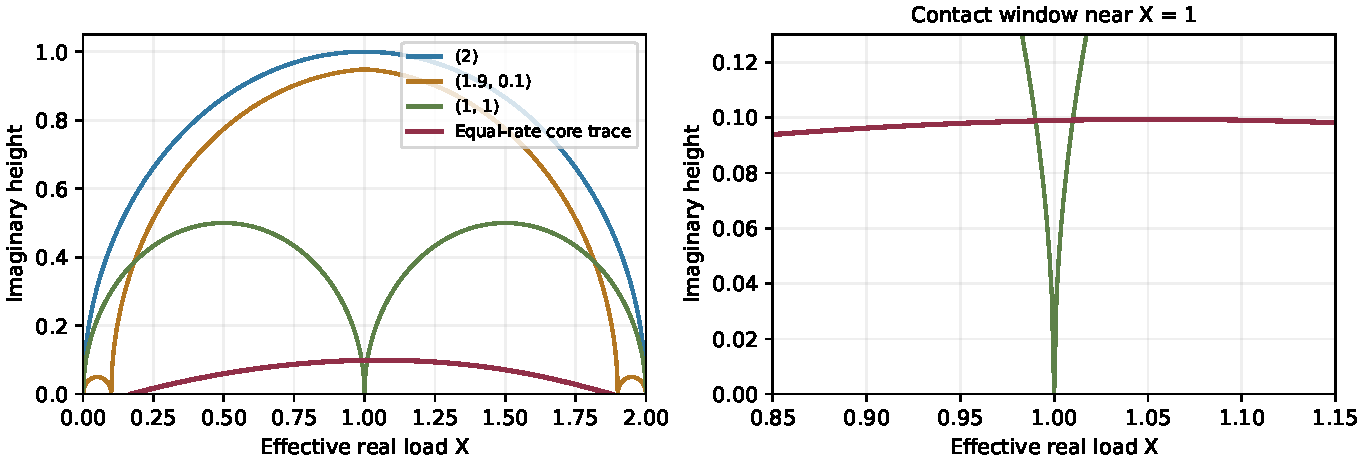
\includegraphics[width=\textwidth]{figures/partition_protection.pdf}
\caption{Partition protection envelopes and an illustrative equal-inner-rate
core trace for $B(6)$. The right panel enlarges the contact near $X=1$.
The red trace is a subset of the core value set, not a certified plot of
the supremum $Q^*$. The stable verdicts use exact edge certificates rather
than an inference from this sampled trace.}
\end{figure}

For $(1,1)$ a finite witness is
\[
 D=\diag(617/1000,617/1000,617/1000,35,158/5,4/125).
\]
The characteristic polynomial has coefficients, in descending order,
\begin{gather*}
 1,\quad \frac{243483}{1000},\quad\frac{29034069433}{5000000},\quad
 \frac{63896127507669}{12500000000},\\
 \frac{36179911928121089}{6250000000000},\quad
 \frac{76473766154601901}{15625000000000},\quad
 \frac{3507069622203}{3906250000000}.
\end{gather*}
Its exact Routh first-column signs are $+,+,+,+,-,+,+$, with no zero
pivots: there are two strictly right-half-plane roots. All coefficients
are positive, so the unstable roots are nonreal. The achieved rate spread
is $\max D_{ii}/\min D_{ii}=4375/4=1093.75$; no optimality is claimed.

For reproducibility of the stable verdicts, the terminal single-leaf
matrix with damping $h$ and gain $g$ has coefficients
\begin{align*}
 1,\quad&c_1+w,\quad c_2+w[p+(h-g)v],\\
 &c_3+w[\tfrac{19}{5}q+(h-g-\tfrac{14}{5})vp],\\
 &c_4+w[\tfrac{466}{25}r+(\tfrac{19}{5}(h-g)-\tfrac{371}{25})vq],\\
 &w[\tfrac{466}{25}(h-g)-\tfrac{18613}{250}]vr.
\end{align*}
For $(h,g)=(6,2)$ and each of the four pairs
\[
 (6,19/10),\quad(59/10,19/10),\quad(6,1/10),\quad(41/10,1/10),
\]
form
$\Delta_k=\det(a_{2j-i+1})_{i,j=0}^{k-1}$ for $k=1,\ldots,4$, with
$a_0=1$ and missing coefficients zero. Substitution
$x=a+b+c$, $y=b+c$, $z=c$ gives only nonnegative rational coefficients,
and a positive polynomial at $a=b=0$. Permutation symmetry of $p,q,r$
covers every ordering of the inner rates. The fifth determinant is
$a_5\Delta_4>0$.

The four edges suffice for the two-leaf verdict: a violating response lies
strictly above a minimizing semicircle in \eqref{eq:envelope}. An interior
point of that semicircle gives a contact for its one-leaf edge, with the
other leaves fixed at their static endpoint loads. At a semicircle endpoint
it gives an imaginary contact for the corresponding static corner.
All these edges and corners are D-stable here. The full determinant is
that of $B(4)$ and has positive sign. Theorem~\ref{thm:partition} applies.
Together with Proposition~\ref{prop:small}, this establishes the four-state
minimum for the fixed-core question.

\section{Buffers, decoys, and what the theorem predicts}
A linear reversible site with binding coefficient $k>0$, unbinding $u>0$,
and bound-complex degradation $\delta\ge0$ contributes a port loss $k$
and positive load
\[
 r=\frac{ku}{u+\delta}.
\]
For a fixed linearized core the relevant static loading interval is therefore
the reachable damping interval from the loss-only core to the fast-site
Schur complement. If both endpoints are D-stable but its interior contains
strict growth, sufficiently fine heterogeneous site classes reveal that
hidden instability. In general the criterion is reachable static growth;
two stable endpoints, and hence literal reentry, are extra hypotheses.

For example, adding total binding loss two to $B(4)$ produces $B(6)$.
With no bound degradation the return total is two. The preceding example
distinguishes one site class, two unequal classes, and two equal classes
under independent positive rates. This is an exact linear interface
example, not a calibrated biochemical clock.

Decoy-induced creation and suppression of oscillations are already known
in nonlinear biomolecular-clock models \cite{dey,karapetyan}; they are not
novel phenomena claimed here. Nonlinear site addition can change the
equilibrium and the core Jacobian, whereas our comparison holds that
Jacobian fixed. In particular a fixed three-state Goodwin core cannot
serve as the four-state granularity example. The conversion from row-rate
freedom to physically linked kinetic parameters must also be checked in
each application.

The maximum of $Q^*$ alone cannot bound the full rate spread needed for
instability: it omits the inner rates attaining that height. A quantitative
statement must retain a core response witness and its rates. The construction
in Lemma~\ref{lem:finite} does so. The rational example above gives an
achieved spread, not a universal ``fragility index'' or a minimum-spread
certificate.

\section{Verification and limits}\label{sec:formal}
Theorem~\ref{thm:threshold}, including $0\le\tau\le-B_{pp}$ and its complete
equality case, is verified end-to-end in Lean against the frozen mathlib
environment. The exported theorem is \texttt{granularity\_threshold} in
the namespace \texttt{DStabilityCharacterization.Granularity}, defined in
\texttt{Threshold.lean}. It uses literal matrix eigenpairs under every
positive diagonal scaling, for arbitrary finite core and leaf index sets.
The tolerance in the converse is quantified before the leaf set and partition.

The proof imports the actual matrix absorption and zero-endpoint theorems,
the contact perturbation of Lemma~\ref{lem:marginal}, the uniform finite
realization of Lemma~\ref{lem:finite}, and the trace argument bounding the
threshold. No spectral-continuation, coverage or realization premise is
assumed. Strict compilation treats warnings as errors, contains no proof
placeholders, and the exported theorem depends only on Lean's standard
axioms \texttt{propext}, \texttt{Classical.choice}, and \texttt{Quot.sound}.

The additional hub, fixed-partition, multiport, reciprocal and
minimum-dimension results have conventional proofs here. Their full formal
assembly, including multiaffine propagation, positive-residue decomposition,
and envelope geometry, is not claimed. Exact rational symbolic replay checks
the examples and polynomial certificates; their generic fifth- and sixth-order
Routh implications are not represented as Lean spectral theorems.

The exact threshold and envelope are reductions. General static D-stability,
computable envelopes for arbitrary interiors, and non-coordinate interfaces
remain outside the scope. The numerical examples establish linear spectral
growth; they do not prove a nonlinear Hopf bifurcation or a stable limit cycle.

\begin{thebibliography}{9}
\bibitem{barmish} B. R. Barmish, \emph{New Tools for Robustness of Linear
Systems}, Macmillan, 1994. Zero-exclusion and value-set methods.
\bibitem{cross} G. W. Cross, Three types of matrix stability,
\emph{Linear Algebra Appl.} \textbf{20} (1978), 253--263.
\href{https://doi.org/10.1016/0024-3795(78)90021-6}{doi:10.1016/0024-3795(78)90021-6}.
\bibitem{lanzon} A. Lanzon and I. R. Petersen, Stability robustness of a
feedback interconnection of systems with negative imaginary frequency
response, \emph{IEEE Trans. Automat. Control} \textbf{53} (2008), 1042--1046.
\href{https://doi.org/10.1109/TAC.2008.919567}{doi:10.1109/TAC.2008.919567}.
\bibitem{willems} J. C. Willems, Realization of systems with internal
passivity and symmetry constraints, \emph{J. Franklin Inst.}
\textbf{301} (1976), 605--621.
\bibitem{chaffey} T. Chaffey, H. J. van Waarde and R. Sepulchre,
Relaxation systems and cyclic monotonicity,
\href{https://arxiv.org/abs/2312.03389}{arXiv:2312.03389}.
\bibitem{dey} S. Dey and A. Singh, Diverse role of decoys on emergence and
precision of oscillations in a biomolecular clock,
\emph{Biophys. J.} \textbf{120} (2021), 5564--5574.
\href{https://doi.org/10.1016/j.bpj.2021.11.013}{doi:10.1016/j.bpj.2021.11.013}.
\bibitem{karapetyan} S. Karapetyan and N. E. Buchler, Role of DNA binding
sites and slow unbinding kinetics in titration-based oscillators,
\href{https://arxiv.org/abs/1509.07420}{arXiv:1509.07420}.
\end{thebibliography}
\end{document}
